
\documentclass[conference]{IEEEtran}

%\usepackage[retainorgcmds]{IEEEtrantools}

\usepackage{cite}
\usepackage{amsmath,amssymb,amsfonts}
\usepackage{algorithmic}
\usepackage{graphicx}
\usepackage{textcomp}
\usepackage{bm}
\usepackage{upgreek}

\usepackage{hyperref}




%\graphicspath{ {C:/Users/Paul/Documents/PhD/Dissertation/Documentation/Figures/} }
\graphicspath{ {../Figures/} }


\DeclareMathOperator*{\argmin}{arg\,min}
\DeclareMathOperator*{\argmax}{arg\,max}

\DeclareMathOperator{\xrm}{\mathrm{x}}
\DeclareMathOperator{\Xrm}{\mathrm{X}}
\DeclareMathOperator{\yrm}{\mathrm{y}}
\DeclareMathOperator{\Yrm}{\mathrm{Y}}
\DeclareMathOperator{\Drm}{\mathrm{D}}
\DeclareMathOperator{\nrm}{\mathrm{n}}
\DeclareMathOperator{\nbarrm}{\bar{\mathrm{n}}}
\DeclareMathOperator{\zrm}{\mathrm{z}}

\DeclareMathOperator{\Prm}{\mathrm{P}}
\DeclareMathOperator{\prm}{\mathrm{p}}
\DeclareMathOperator{\Erm}{\mathrm{E}}
\DeclareMathOperator{\Crm}{\mathrm{C}}

\DeclareMathOperator{\Xcal}{\mathcal{X}}
\DeclareMathOperator{\Ycal}{\mathcal{Y}}
\DeclareMathOperator{\Dcal}{\mathcal{D}}
\DeclareMathOperator{\Ncal}{\mathcal{N}}
\DeclareMathOperator{\Zcal}{\mathcal{Z}}
\DeclareMathOperator{\Hcal}{\mathcal{H}}
\DeclareMathOperator{\Fcal}{\mathcal{F}}
\DeclareMathOperator{\Rcal}{\mathcal{R}}
\DeclareMathOperator{\Mcal}{\mathcal{M}}
\DeclareMathOperator{\Scal}{\mathcal{S}}
\DeclareMathOperator{\Pcal}{\mathcal{P}}
\DeclareMathOperator{\Lcal}{\mathcal{L}}

\DeclareMathOperator{\Rbb}{\mathbb{R}}
\DeclareMathOperator{\Nbb}{\mathbb{N}}
\DeclareMathOperator{\Zbb}{\mathbb{Z}}

\DeclareMathOperator{\Dir}{\mathrm{Dir}}
\DeclareMathOperator{\DM}{\mathrm{DM}}
\DeclareMathOperator{\Mult}{\mathrm{Mult}}
\DeclareMathOperator{\DP}{\mathrm{DP}}
\DeclareMathOperator{\DMP}{\mathrm{DMP}}






\title{Bayesian Learning for Classification using a Uniform Dirichlet Prior}

\author{
\IEEEauthorblockN{Paul Rademacher}
\IEEEauthorblockA{\textit{Radar Division}\\ \textit{U.S. Naval Research Laboratory}\\ Washington, DC, USA\\ paul.rademacher@nrl.navy.mil}
\and
\IEEEauthorblockN{Milo\v{s} Doroslova\v{c}ki}
\IEEEauthorblockA{\textit{Department of Electrical and Computer Engineering}\\ \textit{The George Washington University}\\ Washington, DC, USA\\ doroslov@gwu.edu}
}







\begin{document}

\maketitle

\begin{abstract}
In Bayesian learning, designs based on non-informative priors are appropriate when the user cannot confidently identify the data-generating distribution. While such learners cannot achieve the performance of those based on a well-matched subjective prior, they impart a robustness against poor prior selection. The uniform Dirichlet distribution is the true non-informative prior as it has full support over the space of candidate distributions; additionally, it leads to closed-form posteriors. This work applies such a prior to classification using the 0--1 loss, determines the optimal Bayes classifier and the corresponding minimum probability of error, and analyzes the results.
\end{abstract}

\begin{IEEEkeywords}
Bayesian learning, machine learning, classification, Dirichlet distribution, predictive distribution
\end{IEEEkeywords}




\section{Introduction}

Bayesian approaches to machine learning attempt to make better decisions by exploiting prior knowledge regarding the data-generating distribution. A prior probability distribution weights the different data distributions and defines the mechanism for prediction of unknown quantities using independent training data. When highly concentrated ``subjective'' priors are used, the performance of the learned functions can vary widely \cite{box}. If the prior is localized around the true data-generating model, low-risk decisions can be made even with limited training data; conversely, if the prior assigns low weighting to the true model, satisfactory performance may not be realized. 

If the designer does not have prior confidence in any specific model, a non-informative prior distribution can be used to weight the different models equally. Although learners designed with such priors will not perform as well as those made with well-selected subjective priors, they provide a robust solution regardless of the model. Often, priors are termed non-informative as long as they are approximately uniform over their support. The uniform Dirichlet distribution is unique in that it has full support over the space of data-generating distributions and is thus truly non-informative. Additionally, it is a conjugate prior \cite{theodoridis-ML} for independent, identically distributed observations and leads to a closed-form model posterior distribution.

This work assumes that joint observed/unobserved random variables are drawn from finite sets, enabling the use of the uniform Dirichlet prior. After discussing the relevant probability distributions, they will be applied to Bayesian classification using the 0--1 loss function \cite{berger}. The effects of the data set cardinalities and the volume of training data on the minimum probability of error will be analyzed and discussed.







\section{Objective}

Consider an observable random element $\xrm \in \Xcal$ and and unobservable random element $\yrm \in \Ycal$ which are jointly distributed according to an unknown probability mass function (PMF) $\theta \in \Theta = \left\{ \theta \in {\Rbb_{\geq 0}}^{\Ycal \times \Xcal}: \sum_{y \in \Ycal} \sum_{x \in \Xcal} \theta(y,x) = 1 \right\}$, such that $\Prm_{\yrm,\xrm | \uptheta}(y,x | \theta) = \theta(y,x)$. 

Also observed is a random sequence of $N$ samples drawn from $\theta$, denoted $\Drm \in \Dcal = \{\Ycal \times \Xcal\}^N$. The $N$ data pairs are identically distributed as $\Prm_{\Drm_n | \uptheta}(y,x | \theta) = \theta(y,x)$ and are conditionally independent from one another and from the novel pair $(\yrm,\xrm)$.

The objective is to design a decision function $f: \Dcal \mapsto \Hcal^{\Xcal}$ which outputs a mapping from the space of the observed random element $\xrm$ to a decision space $\Hcal$. The metric guiding the design is a loss function $\Lcal: \Hcal \times \Ycal \mapsto \Rbb_{\geq 0}$ which penalizes the decision $h \in \Hcal$ based on the value of $\yrm$. The conditional expected loss, or conditional ``risk'', is defined as
\begin{equation} \label{eq:risk_cond}
\Rcal_{\Theta}(f ; \uptheta) = \Erm_{\xrm,\Drm | \uptheta} \bigg[ \Erm_{\yrm | \xrm,\uptheta} \Big[ \Lcal\big( f(\xrm;\Drm),\yrm \big) \Big] \bigg] \;.
\end{equation}

As the model $\theta$ is not observed, $\Rcal_{\Theta}$ is not yet a feasible objective function for optimization. If the designer selects a probability density function (PDF) $\prm_{\uptheta}$, the Bayes risk is formulated as
\begin{IEEEeqnarray}{rCl} \label{eq:risk}
\Rcal(f) & = & \Erm_{\uptheta}\big[ \Rcal_{\Theta}(f ; \uptheta) \big] \\
& = & \Erm_{\xrm,\Drm}\bigg[ \Erm_{\yrm | \xrm,\Drm} \Big[ \Lcal\big( f(\xrm;\Drm),\yrm \big) \Big] \bigg] \nonumber
\end{IEEEeqnarray}
and $\yrm$, $\xrm$, and $\Drm$ are treated as jointly distributed random elements. The optimal learning function is expressed as
\begin{equation} \label{eq:f_opt_xD}
f^*(\xrm;\Drm) = \argmin_{h \in \Hcal} \Erm_{\yrm | \xrm,\Drm}\big[ \Lcal(h,\yrm) \big]
\end{equation}
and the corresponding minimum Bayes risk is
\begin{equation} \label{eq:risk_min}
\Rcal(f^*) = \Erm_{\xrm,\Drm} \left[ \min_{h \in \Hcal} \Erm_{\yrm | \xrm,\Drm}\big[ \Lcal(h,\yrm) \big] \right] \;.
\end{equation}














\section{Probability Distributions}

In this section, the joint PMF $\Prm_{\yrm,\xrm,\Drm}$ is determined using the uniform Dirichlet prior $\prm_{\uptheta}$. Other distributions of interest will be provided, including the training data PMF $\Prm_{\Drm}$ and the predictive distribution $\Prm_{\yrm | \xrm,\Drm}$.




\subsection{Model PDF, $\prm_{\uptheta}$} \label{sec:P_theta}

The uniform PDF of the model random process $\uptheta \in \Theta$ is Dirichlet \cite{bishop} with parameters $\alpha(\cdot,\cdot) = 1$, such that
\begin{IEEEeqnarray}{rCl}
\prm_{\uptheta}(\theta) & = & \bigg[ \beta(\alpha)^{-1} \prod_{y \in \Ycal} \prod_{x \in \Xcal} \theta(y,x)^{\alpha(y,x) - 1} \bigg]_{\alpha(\cdot,\cdot) = 1} \\
& = & \big( |\Ycal||\Xcal|-1 \big)! \nonumber 
\end{IEEEeqnarray}
is uniform over $\Theta$. The operator $\beta$ is the generalized beta function and $!$ denotes the factorial. 


%Figure \ref{fig:P_theta_uniform} shows the uniform distribution amplitude for $|\Ycal| = 3$ and $|\Xcal| = 1$.
%
%\begin{figure}
%\centering
%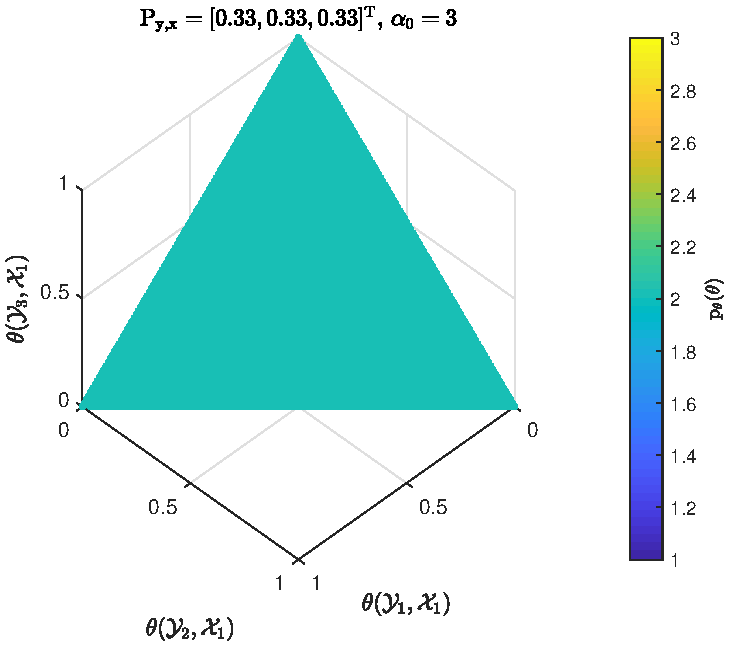
\includegraphics[width=0.9\linewidth]{P_theta_uniform.pdf}
%\caption{Uniform model prior PDF, $|\Ycal| = 3$, $|\Xcal| = 1$}
%\label{fig:P_theta_uniform}
%\end{figure}

For convenience, the Dirichlet concentration parameter is defined as $\alpha_0 \equiv \sum_{y \in \Ycal} \sum_{x \in \Xcal} \alpha(y,x)$. The mean function of the model is 
\begin{equation}
\mu_{\uptheta}(y,x) = \frac{\alpha(y,x)}{\alpha_0}\bigg|_{\alpha(\cdot,\cdot) = 1} = \big( |\Ycal||\Xcal| \big)^{-1} \;.
\end{equation}
The marginal data PMF $\Prm_{\yrm,\xrm} = \mu_{\uptheta}$ is uniform over $\Ycal \times \Xcal$. 













\subsection{Training Set PMF, $\Prm_{\Drm}$}

Next, the conditional distribution $\Prm_{\Drm | \uptheta}$ will be used to determine the marginal training data PMF, $\Prm_{\Drm}$. The distribution of $\Drm$ conditioned on the model can be formulated as
\begin{IEEEeqnarray}{rCl}
\Prm_{\Drm | \uptheta}(D | \theta) & = & \prod_{y \in \Ycal} \prod_{x \in \Xcal} \theta(y,x)^{\bar{N}(y,x;D)} \;,
\end{IEEEeqnarray}
where the dependency on the training data $\Drm$ is expressed though a transform function $\bar{N} : \Dcal \mapsto \bar{\Ncal}$, defined as $\bar{N}(y,x;D) = \sum_{n=1}^N \delta\big[ (y,x),D_n \big]$, which counts the number of occurrences of the pair $(y,x)$ in the training set $D$. The range of the transform is the function space $\bar{\Ncal} = \left\{ \bar{n} \in {\Zbb_{\geq 0}}^{\Ycal \times \Xcal}: \sum_{y \in \Ycal} \sum_{x \in \Xcal} \bar{n}(y,x) = N \right\}$. The cardinality of the set is $|\bar{\Ncal}| = \binom{N+|\Ycal||\Xcal|-1}{|\Ycal||\Xcal|-1}$; this can be shown using the stars-and-bars method \cite{feller}.

Note that $\Prm_{\Drm | \uptheta}$ depends on the training data $\Drm$ only through the transform $\bar{N}$; $\bar{N}(\Drm)$ is thus a sufficient statistic \cite{bernardo} for the model $\uptheta$. Consequently, other distributions of interest $\Prm_{\Drm}$ and $\Prm_{\yrm | \xrm,\Drm}$ will also depend on $\Drm$ via $\bar{N}(\Drm)$. As such, it is useful to define a new random process $\nbarrm \equiv \bar{N}(\Drm) \in \bar{\Ncal}$. 

The conditional PMF $\Prm_{\nbarrm | \uptheta}$ is easily shown to be Multinomial. As a Dirichlet distribution $\prm_{\uptheta}$ characterizes the parameters of this distribution, the marginal PMF of $\nbarrm$ is a Dirichlet-Multinomial distribution \cite{johnson} parameterized by $\alpha(\cdot,\cdot) = 1$,
\begin{IEEEeqnarray}{rCl}
\Prm_{\nbarrm}(\bar{n}) & = & \Mcal(\bar{n}) \beta(\alpha)^{-1} \beta(\alpha + \bar{n}) \big|_{\alpha(\cdot,\cdot) = 1} \\
& = & |\bar{\Ncal}|^{-1} = \binom{N+|\Ycal||\Xcal|-1}{|\Ycal||\Xcal|-1}^{-1} \nonumber \;,
\end{IEEEeqnarray}
which is uniform over the set $\bar{\Ncal}$. The operator $\Mcal$ represents the multinomial coefficient.












\subsection{Predictive PMF, $\Prm_{\yrm | \xrm,\Drm}$}

As shown in Equation \eqref{eq:f_opt_xD}, the decision selected by the optimally designed function depends on the Bayesian predictive PMF $\Prm_{\yrm | \xrm,\Drm}$. First, note that as $\Prm_{\Drm | \uptheta}$ is of exponential form, the Dirichlet PDF $\prm_{\uptheta}$ is its conjugate prior \cite{theodoridis-ML}; thus, the posterior PDF $\prm_{\uptheta | \Drm}$ is a Dirichlet distribution with parameter function $\alpha(y,x) = \bar{N}(y,x;\Drm) + 1$,
\begin{IEEEeqnarray}{rCl}
\prm_{\uptheta | \Drm}(\theta | D) & = & \big(N+|\Ycal||\Xcal|-1\big)! \\
&& \qquad \times \prod_{y \in \Ycal} \prod_{x \in \Xcal} \frac{\theta(y,x)^{\bar{N}(y,x;\Drm)}}{\bar{N}(y,x;\Drm)!} \nonumber \;.
\end{IEEEeqnarray}
The posterior concentration parameter is $\alpha_0 = N+|\Ycal||\Xcal|$; Figure \ref{fig:P_theta_post_uni} shows how the posterior is localized around the empirical PMF $\bar{N}(\Drm)/N$ when the model is conditioned on the training data.
%The posterior concentration parameter is $\alpha_0 = N+|\Ycal||\Xcal|$; Figure \ref{fig:P_theta_post_uni} shows how the posterior tends toward $\prm_{\uptheta}(\theta) \to \delta\big( \theta - \mu_{\uptheta} \big) = \delta\big( \theta - \bar{N}(\Drm)/N \big)$ with infinite training data.

\begin{figure}
\centering
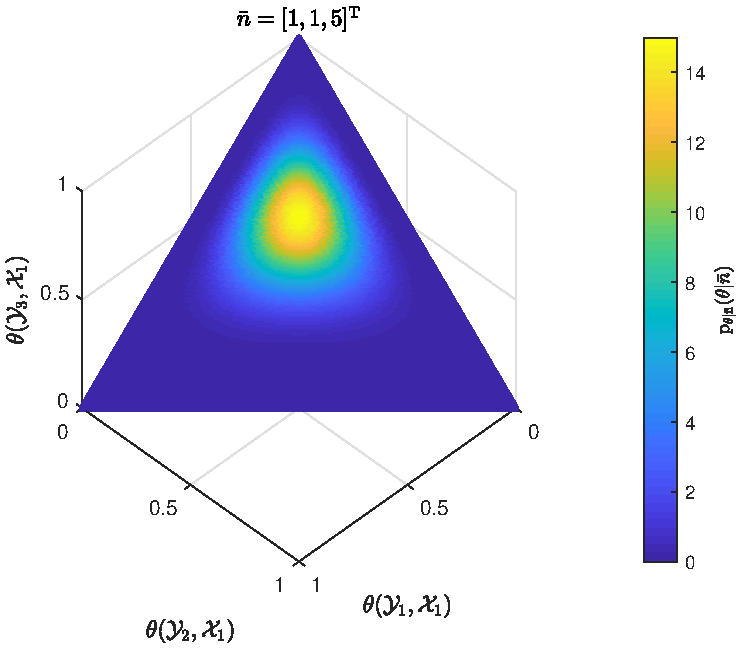
\includegraphics[width=0.9\linewidth]{P_theta_post_uni.pdf}
\caption{Model Posterior for an example training set $\nbarrm$}
\label{fig:P_theta_post_uni}
\end{figure}


The joint PMF of $\yrm$ and $\xrm$ conditioned on the training data is expressed as $\Prm_{\yrm,\xrm | \Drm} = \mu_{\uptheta | \Drm}$ \cite{murphy}. The predictive distribution of interest is generated via Bayes rule as
\begin{IEEEeqnarray}{rCl} \label{P_y_xD_uniform}
\Prm_{\yrm | \xrm,\Drm}(y | x,D) & = & \frac{\bar{N}(y,x;D)+1}{N'(x;D) + |\Ycal|} \\
& = & \left( \frac{|\Ycal|}{N'(x;D) + |\Ycal|} \right) \frac{1}{|\Ycal|} \nonumber \\
&& \quad + \left( \frac{N'(x;D)}{N'(x;D) + |\Ycal|} \right) \frac{\bar{N}(y,x;D)}{N'(x;D)} \nonumber \;,
\end{IEEEeqnarray}
where $N'(x;D) = \sum_{y \in \Ycal} \bar{N}(y,x;D)$.

The second form represents the predictive PMF as a convex combination of two conditional distributions. The first PMF $\Prm_{\yrm | \xrm} = |\Ycal|^{-1}$ is uniform and independent of the training data; the second distribution is the conditional empirical PMF. As the number of matching training data $N'(x;\Drm)$ increases relative to the number of classes $|\Ycal|$, the predictive PMF tends toward the empirical PMF.









\section{Classification using the 0--1 Loss}

In this section, the developed framework is applied to classification. The 0--1 loss function is the most widely used for these problems; it is represented as $\Lcal(h,y) = 1 - \delta[h,y]$ with hypothesis space $\Hcal = \Ycal$.


\subsection{Optimal Hypothesis: the Conditional Majority Decision}

To determine the optimal learning function, the 0--1 loss is substituted into \eqref{eq:f_opt_xD} to find
\begin{IEEEeqnarray}{rCl} \label{eq:f_opt_01}
f^*(\xrm;\Drm) & = & \argmin_{h \in \Ycal} \Erm_{\yrm | \xrm,\Drm}\big[ 1 - \delta[h,\yrm] \big] \\
& = & \argmax_{y \in \Ycal} \Prm_{\yrm | \xrm,\Drm}(y | \xrm,\Drm) \nonumber \\
& = & \argmax_{y \in \Ycal} \bar{N}(y,\xrm;\Drm) \nonumber \;.
\end{IEEEeqnarray}
The optimal classifier chooses the value $y \in \Ycal$ that maximizes the predictive PMF given the observed values of $\xrm$ and $\Drm$. It is a conditional majority decision which chooses the class from $\Ycal$ most often represented among training set samples $\Drm$ with a matching input value $\xrm = x$. 







\subsection{Minimum Bayes Probability of Error}

Substituting the 0--1 loss into \eqref{eq:risk_min}, the minimum Bayes 0--1 risk is 
\begin{IEEEeqnarray}{rCl}
\Rcal^* & = & 1 - \Erm_{\xrm,\Drm} \left[ \max_{y \in \Ycal} \Prm_{\yrm | \xrm,\Drm}(y | \xrm,\Drm) \right] \\
& = & 1 - \sum_{x \in \Xcal} \frac{\Erm_{\nbarrm} \big[ \max_{y \in \Ycal} \bar{\nrm}(y,x) \big] + 1}{|\Ycal||\Xcal| + N} \nonumber \;.
\end{IEEEeqnarray}
The expectation operates on the maximum value from a subset of the random process $\nbarrm$ -- it is found in Appendix \ref{app:n_max}. Substituting, the minimum 0--1 Bayes risk is
\begin{IEEEeqnarray}{L}
\Rcal^* = 1 - \big(|\Ycal| + N/|\Xcal|\big)^{-1} \\
\qquad \times \sum_{m=1}^{|\Ycal|} \binom{|\Ycal|}{m} (-1)^{m-1} \sum_{n=0}^{\big\lfloor\frac{N}{m}\big\rfloor} \prod_{l=1}^{|\Ycal||\Xcal|-1} \Big( 1-\frac{mn}{N+l} \Big) \nonumber \; .
\end{IEEEeqnarray}
%\begin{IEEEeqnarray}{rCl}
%\Rcal^* & = & 1 - \frac{\sum_{m=1}^{|\Ycal|} \binom{|\Ycal|}{m} (-1)^{m-1} \sum_{n=0}^{\big\lfloor\frac{N}{m}\big\rfloor} \prod_{l=1}^{|\Ycal||\Xcal|-1} \Big( 1-\frac{mn}{N+l} \Big)}{|\Ycal| + N/|\Xcal|} \; .
%\end{IEEEeqnarray}
%\begin{IEEEeqnarray}{L}
%\Rcal^* = 1 - \\
%\quad \frac{\sum_{m=1}^{|\Ycal|} \binom{|\Ycal|}{m} (-1)^{m-1} \sum_{n=0}^{\big\lfloor\frac{N}{m}\big\rfloor} \prod_{l=1}^{|\Ycal||\Xcal|-1} \Big( 1-\frac{mn}{N+l} \Big)}{|\Ycal| + N/|\Xcal|} \nonumber \; .
%\end{IEEEeqnarray}

It is informative to express the risk for minimal and maximal volumes of training data. Using an identity for alternating binomial sums of polynomials \cite{graham}, it can be shown that for $N = 0$, the minimum risk is $\Rcal^*  = 1 - |\Ycal|^{-1}$. 

To find the risk for $N \to \infty$, note that
\begin{IEEEeqnarray}{L}
\lim_{N \to \infty} \big( |\Ycal| + N/|\Xcal| \big)^{-1} \sum_{n=0}^{\big\lfloor\frac{N}{m}\big\rfloor} \prod_{l=1}^{|\Ycal||\Xcal|-1} \Big( 1-\frac{mn}{N+l} \Big) \quad \\
\qquad = \lim_{N/m \to \infty} \frac{|\Xcal|}{N} \sum_{n=0}^{\big\lfloor\frac{N}{m}\big\rfloor} \left( 1 - \frac{mn}{N} \right)^{|\Ycal||\Xcal|-1} \nonumber \\
\qquad = \frac{|\Xcal|}{m} \int_0^1 (1-t)^{|\Ycal||\Xcal|-1} \mathrm{d} t  = \frac{1}{m|\Ycal|} \nonumber \;.
\end{IEEEeqnarray}
Thus, the 0--1 Bayes risk for the uniform prior tends toward
\begin{IEEEeqnarray}{rCl}
\Rcal^* & \to & 1 - |\Ycal|^{-1} \sum_{m=1}^{|\Ycal|} \binom{|\Ycal|}{m} (-1)^{m-1} m^{-1} \\
& = & 1 - |\Ycal|^{-1} \sum_{m=1}^{|\Ycal|} m^{-1} \nonumber \;,
\end{IEEEeqnarray}
providing a lower bound for the achievable Bayes probability of error. The above formulation has made use of the alternating summation identity from \cite{roman} to express the risk using the $|\Ycal|^\mathrm{th}$ harmonic number $H_{|\Ycal|} = \sum_{m=1}^{|\Ycal|} m^{-1}$. Observe that the risk does not depend on the cardinality $|\Xcal|$.


Figures \ref{fig:Risk_01_uni_N_leg_My} and \ref{fig:Risk_01_uni_N_leg_Mx} demonstrate how the minimum 0--1 risk decreases with training volume $N$ for different cardinalities $|\Ycal|$ and $|\Xcal|$ respectively. With a larger set of classes, accurate classification becomes more difficult; similarly, the probability of error increases with the number of possible observations $\xrm = x$. 


\begin{figure}
\centering
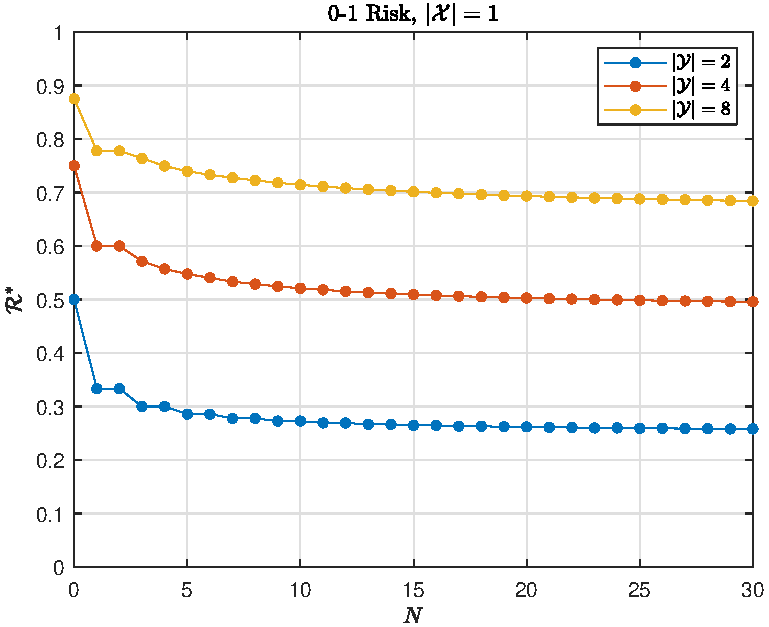
\includegraphics[width=0.9\linewidth]{Risk_01_uni_N_leg_My.pdf}
\caption{Minimum 0--1 Risk for different numbers of classes}
\label{fig:Risk_01_uni_N_leg_My}
\end{figure}

\begin{figure}
\centering
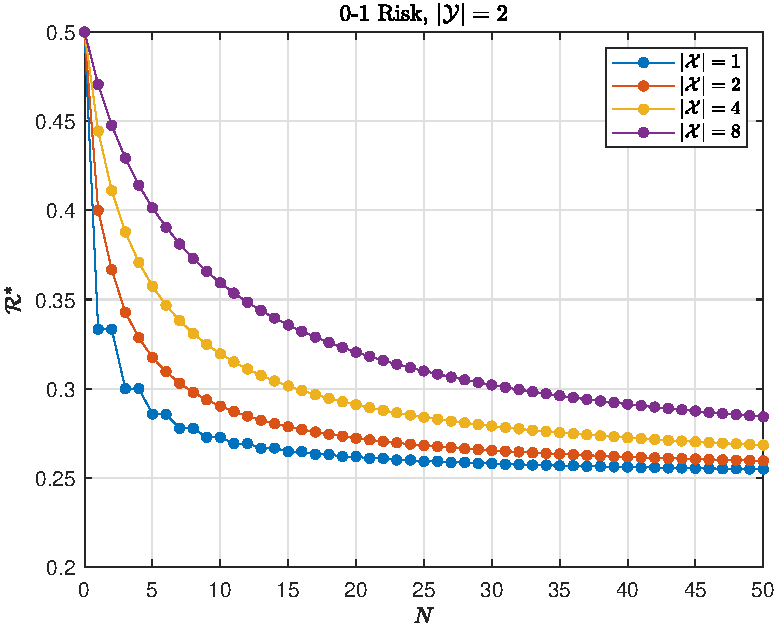
\includegraphics[width=0.9\linewidth]{Risk_01_uni_N_leg_Mx.pdf}
\caption{Minimum 0--1 Risk for different numbers of possible observations}
\label{fig:Risk_01_uni_N_leg_Mx}
\end{figure}

Further insight into how the risk depends on $|\Xcal|$ is obtained by plotting the risk as a function of $N/|\Xcal|$. In Figure \ref{fig:Risk_01_uni_N-Mx}, it is shown that the optimal risk can be approximated by a function dependent only on $N/|\Xcal|$; of the series plotted, only the series for $|\Xcal| = 1$ shows non-negligible deviation from the others.

\begin{figure}
\centering
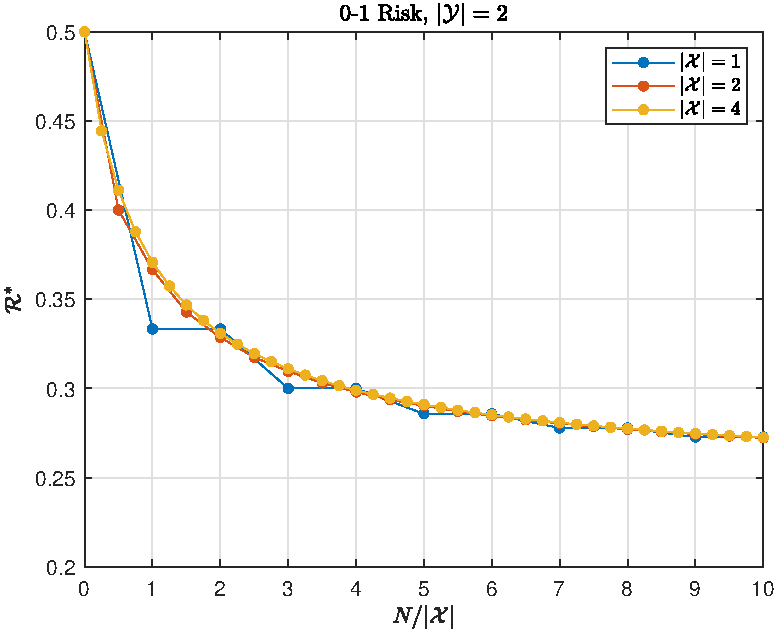
\includegraphics[width=0.9\linewidth]{Risk_01_uni_N-Mx.pdf}
\caption{Minimum 0--1 Risk as a function of $N/|\Xcal|$}
\label{fig:Risk_01_uni_N-Mx}
\end{figure}


It is also informative to graph the $N=0$ and $N \to \infty$ minimum risk values as a function of $|\Ycal|$. Figure \ref{fig:Risk_01_uni_N_bounds} displays these bounds; note the margin in the probability of error between the optimal $N=0$ and $N \to \infty$ classifiers. For binary classification $\big( |\Ycal| = 2 \big)$, infinite training data reduces the expected probability of error from 0.5 to 0.25. As $|\Ycal|$ increases, the classification risk for both sequences tends to unity and any improvement due to training data becomes negligible.

\begin{figure}
\centering
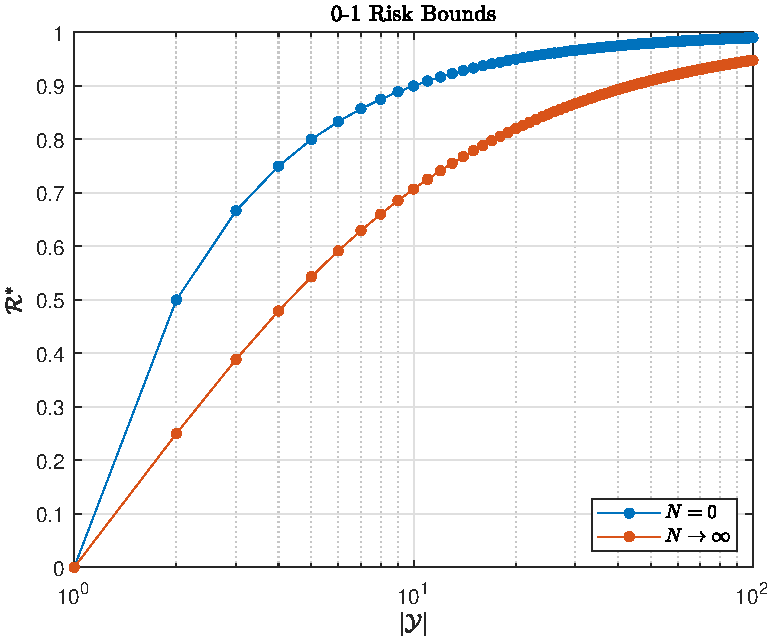
\includegraphics[width=0.9\linewidth]{Risk_01_uni_N_bounds.pdf}
\caption{Minimum 0--1 Risk for zero and infinite number of training data}
\label{fig:Risk_01_uni_N_bounds}
\end{figure}






\section{Conclusion}

This work has used the non-informative uniform Dirichlet prior for Bayesian learning, discussed the Bayes predictive distribution, and applied the results to classification. The optimal majority decision learner and the minimum 0--1 risk have been analyzed. Graphical examples illustrate how the probability of error increases with the number of classes and the number of possible observations. Additionally, the asymptotic Bayes risk using infinite training data has been found and its deviation from the risk of an untrained classifier has been discussed. 

Future work will expand the results presented for a general Dirichlet prior. The effect of the subjectivity of the prior on the conditional risk \eqref{eq:risk_cond} will be of specific interest. Additionally, the work will be generalized for an infinite number of possible observations using Dirichlet processes








\appendices

\section{Evaluation of $\Erm_{\nbarrm} \big[ \max_{y \in \Ycal} \bar{\nrm}(y,x) \big]$} \label{app:n_max}

To evaluate the expectation, new random variables $\nbarrm_{\max}(x) \equiv \max_{y \in \Ycal} \nbarrm(y,x)$ are introduced and characterized by the event probabilities $\Prm\big( \nbarrm_{\max}(x) \geq n \big) = \Prm\big( \cup_{y \in \Ycal} \{ \nbarrm(y,x) \geq n \} \big)$. As the distribution of $\nbarrm$ is uniform, the event probability is proportionate to the cardinality of the set $\cup_{y \in \Ycal} \{ \bar{n}: \bar{n}(y,x) \geq n \}$. Using the inclusion-exclusion principle \cite{brualdi}, the cardinality is represented as
\begin{IEEEeqnarray}{L}
\big| \cup_{y \in \Ycal} \{ \bar{n} : \bar{n}(y,x) \geq n \} \big| \\
\quad = \begin{cases} \binom{N+|\Ycal||\Xcal|-1}{|\Ycal||\Xcal|-1} & \mathrm{if} \ n < 0, \\ \sum_{m=1}^{|\Ycal|} \binom{|\Ycal|}{m} (-1)^{m-1} \\ \; \; \times \binom{N-mn+|\Ycal||\Xcal|-1}{|\Ycal||\Xcal|-1} H\Big( \big\lfloor\frac{N}{m}\big\rfloor - n \Big) & \mathrm{if} \ 0 \leq n \leq N, \\ 0 & \mathrm{if} \ n > N, \end{cases} \nonumber
\end{IEEEeqnarray}
where $H: \Zbb \mapsto \{0,1\}$ is the discrete Heaviside step function. Note the independence from $x$.

For $n < 0$, the cardinality is equivalent to $|\bar{\Ncal}|$. For $0 \leq n < N$, the cardinality is an alternating binomial summation where the $m^\mathrm{th}$ term accounts for the different intersections of $m$ of the $|\Ycal|$ individual sets $\{ \bar{n} : \bar{n}(y,x) \geq n \}$. Observe that the cardinality of the intersections is only dependent on the number of contributing sets $m$ and not on which sets intersect. Furthermore, note the dependency of the intersection cardinalities on the argument $n$. The step function contributes such that if $n > \big\lfloor\frac{N}{m}\big\rfloor$, only up to $m-1$ individual sets will intersect. The binomial coefficient calculates the intersection cardinality for a given $m$; note the similarity to the cardinality $|\bar{\Ncal}|$ - the only difference is the number of points characterizing the $|\Ycal||\Xcal|-1$ dimensional region.

The probability of interest can thus be expressed as $\Prm\big( \nbarrm_{\max}(x) \geq n \big) = |\bar{\Ncal}|^{-1} \ \big| \cup_{y \in \Ycal} \{ \bar{n} : \bar{n}(y,x) \geq n \} \big|$. Since the PMF of $\nbarrm_{\max}(x)$ has support on $n \in [0,\ldots,N]$, the expectation over $\nbarrm$ is evaluated as
\begin{IEEEeqnarray}{L}
\Erm_{\nbarrm}\big[ \nbarrm_{\max}(x) \big] = \sum_{n=0}^N n \Prm\big( \nbarrm_{\max}(x) = n \big) \\
\quad = -1 + \sum_{n=0}^N \Prm\big( \nbarrm_{\max}(x) \geq n \big) \nonumber \\
\quad = -1 + \sum_{m=1}^{|\Ycal|} \binom{|\Ycal|}{m} (-1)^{m-1} \sum_{n=0}^{\big\lfloor\frac{N}{m}\big\rfloor} \prod_{l=1}^{|\Ycal||\Xcal|-1} \Big( 1-\frac{mn}{N+l} \Big) \nonumber \;.
\end{IEEEeqnarray}
%\begin{IEEEeqnarray}{rCl}
%\Erm_{\nbarrm}\big[ \nbarrm_{\max}(x) \big] & = & \sum_{n=0}^N n \Prm\big( \nbarrm_{\max}(x) = n \big) \\
%& = & -1 + \sum_{n=0}^N \Prm\big( \nbarrm_{\max}(x) \geq n \big) \nonumber \\
%& = & -1 + \sum_{m=1}^{|\Ycal|} \binom{|\Ycal|}{m} (-1)^{m-1} \nonumber \\
%&& \qquad \quad \sum_{n=0}^{\big\lfloor\frac{N}{m}\big\rfloor} \prod_{l=1}^{|\Ycal||\Xcal|-1} \Big( 1-\frac{mn}{N+l} \Big) \nonumber \;.
%\end{IEEEeqnarray}
%\begin{IEEEeqnarray}{L}
%\Erm_{\nbarrm}\big[ \nbarrm_{\max}(x) \big] = \sum_{n=0}^N n \Prm\big( \nbarrm_{\max}(x) = n \big) \\
%\quad = -1 + \sum_{n=0}^N \Prm\big( \nbarrm_{\max}(x) \geq n \big) \nonumber \\
%\quad = -1 + |\bar{\Ncal}|^{-1} \sum_{m=1}^{|\Ycal|} \binom{|\Ycal|}{m} (-1)^{m-1} \nonumber \\
%\qquad \qquad \sum_{n=0}^{\big\lfloor\frac{N}{m}\big\rfloor} \binom{N-mn+|\Ycal||\Xcal|-1}{|\Ycal||\Xcal|-1} \nonumber \;.
%\end{IEEEeqnarray}



\bibliographystyle{IEEEtran}
\bibliography{{../References/phd_bib}}


\end{document}


























